\documentclass[11pt,a4paper]{article}

% ── Packages ──────────────────────────────────────────────────────────────────
\usepackage[T1]{fontenc}
\usepackage[utf8]{inputenc}
\usepackage[margin=2.5cm]{geometry}
\usepackage{lmodern}
\usepackage{microtype}
\usepackage{amsmath,amssymb}
\usepackage{booktabs}
\usepackage{array}
\usepackage{multirow}
\usepackage[table,dvipsnames]{xcolor}
\usepackage{graphicx}
\usepackage{float}
\usepackage{caption}
\usepackage{subcaption}
\usepackage{hyperref}
\usepackage{titlesec}
\usepackage{enumitem}
\usepackage{tikz}
\usetikzlibrary{shapes.geometric, arrows.meta, positioning, fit,
                decorations.pathreplacing, backgrounds, calc, shadows}

% ── Colors ────────────────────────────────────────────────────────────────────
\definecolor{cBlue}{HTML}{2563EB}
\definecolor{cGreen}{HTML}{16A34A}
\definecolor{cOrange}{HTML}{EA580C}
\definecolor{cPurple}{HTML}{7C3AED}
\definecolor{cRed}{HTML}{DC2626}
\definecolor{cGray}{HTML}{6B7280}
\definecolor{cLightBlue}{HTML}{DBEAFE}
\definecolor{cLightGreen}{HTML}{DCFCE7}
\definecolor{cLightOrange}{HTML}{FFEDD5}
\definecolor{cLightPurple}{HTML}{EDE9FE}
\definecolor{cLightGray}{HTML}{F3F4F6}
\definecolor{cBestRow}{HTML}{FEF9C3}

% ── TikZ Styles ───────────────────────────────────────────────────────────────
\tikzset{
  box/.style={
    rectangle, rounded corners=4pt, draw=#1!70, fill=#1!12,
    minimum width=2.6cm, minimum height=0.75cm,
    text width=2.5cm, align=center, font=\small\sffamily,
    drop shadow={shadow xshift=0.5pt, shadow yshift=-0.5pt, opacity=0.15}
  },
  wbox/.style={box=cGray, minimum width=3.2cm, text width=3.1cm},
  pbox/.style={box=cBlue},
  gbox/.style={box=cGreen},
  obox/.style={box=cOrange},
  rbox/.style={box=cRed},
  vbox/.style={box=cPurple},
  arrow/.style={-{Stealth[length=5pt]}, thick, #1},
  arrow/.default=cGray,
  darrow/.style={Stealth[length=5pt]-{Stealth[length=5pt]}, thick, cGray},
  label/.style={font=\footnotesize\sffamily\itshape, text=cGray},
}

% ── Section formatting ────────────────────────────────────────────────────────
\titleformat{\section}{\large\bfseries\sffamily}{\thesection}{1em}{}[\vspace{-2pt}\rule{\linewidth}{0.4pt}]
\titleformat{\subsection}{\normalsize\bfseries\sffamily}{\thesubsection}{1em}{}

\hypersetup{colorlinks=true, linkcolor=cBlue, urlcolor=cBlue, citecolor=cBlue}

% ── Title ─────────────────────────────────────────────────────────────────────
\title{%
  \sffamily\LARGE\bfseries
  Allosteric Pocket Prediction via\\
  Continuous-Time Quantum Walk\\[6pt]
  \large\normalfont\sffamily\color{cGray}
  Cleveland Clinic Challenge 2026 --- Technical Report
}
\author{\sffamily Leo}
\date{\sffamily June 2026}

% ══════════════════════════════════════════════════════════════════════════════
\begin{document}
\maketitle
\tableofcontents
\vspace{1em}

% ══════════════════════════════════════════════════════════════════════════════
\section{Problem Statement}

Given only the \textbf{apo (unbound) crystal structure} of a protein, predict which
residues form the \textbf{allosteric pocket}---a distal binding site that modulates
protein function without blocking the active site.

\vspace{0.5em}
\noindent\textbf{Challenge proteins:}

\begin{table}[H]
\centering
\begin{tabular}{llll}
\toprule
\textbf{Protein} & \textbf{Apo PDB} & \textbf{Allosteric ligand} & \textbf{Relevance} \\
\midrule
KRAS G12C       & 4OBE & Sotorasib (6OIM)  & Oncogenic RAS, switch-II pocket \\
BCR-ABL1        & 1OPL & Asciminib (5MO4)  & Leukemia kinase, myristoyl pocket \\
Cardiac Myosin  & 5TBY & Mavacamten (6C1H) & Hypertrophic cardiomyopathy \\
\bottomrule
\end{tabular}
\end{table}

The BCR-ABL1 myristoyl pocket is $>$30\,\r{A} from the ATP-binding active site,
making it unreachable by classical diffusion methods.

% ══════════════════════════════════════════════════════════════════════════════
\section{Core Hypothesis and Overall Pipeline}

\begin{figure}[H]
\centering
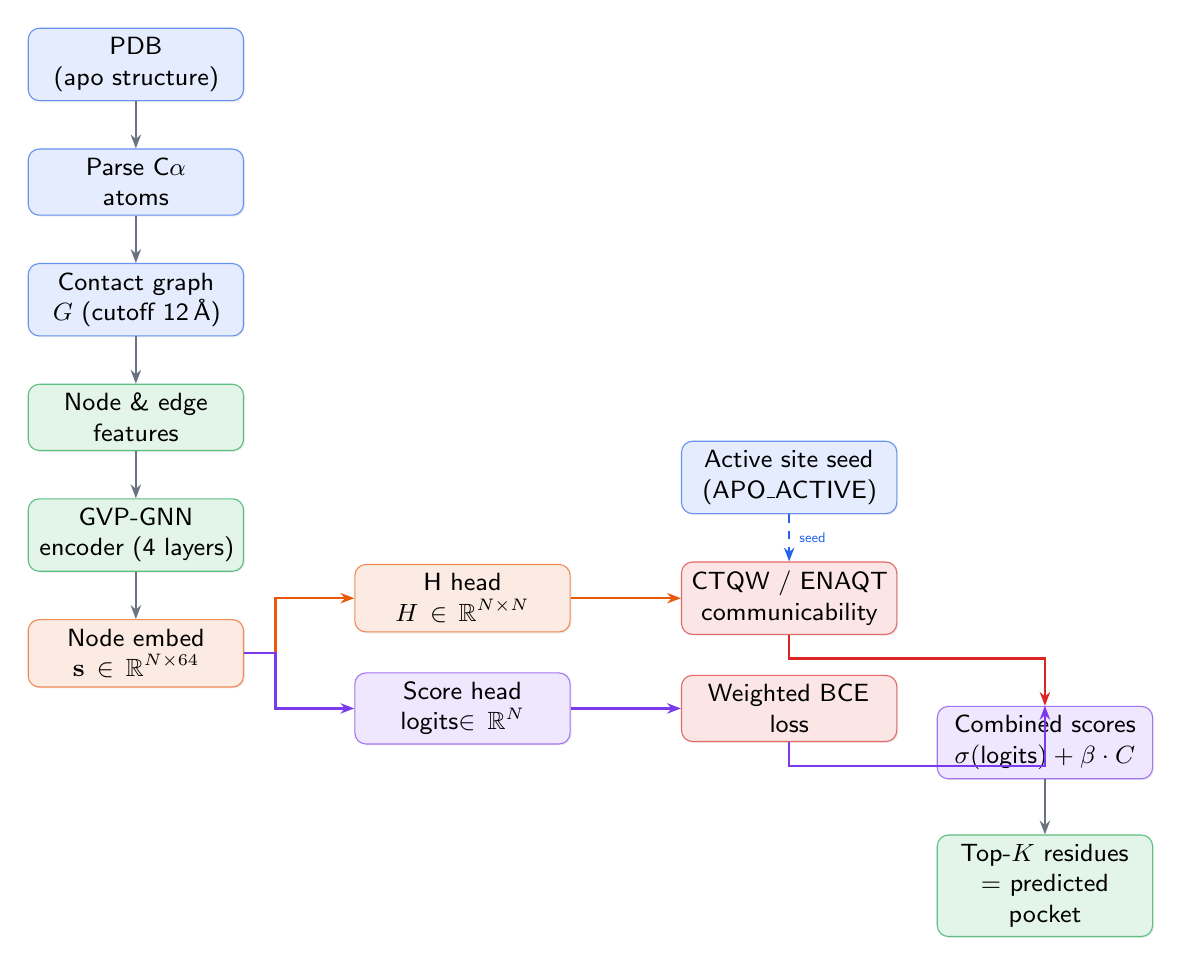
\begin{tikzpicture}[node distance=0.6cm and 1.1cm]

  % Column 1: data pipeline
  \node[pbox] (pdb)   {PDB\\(apo structure)};
  \node[pbox, below=of pdb]   (parse) {Parse C$\alpha$\\atoms};
  \node[pbox, below=of parse] (graph) {Contact graph\\$G$ (cutoff 12\,\r{A})};
  \node[gbox, below=of graph] (feat)  {Node \& edge\\features};
  \node[gbox, below=of feat]  (enc)   {GVP-GNN\\encoder (4 layers)};
  \node[obox, below=of enc]   (embed) {Node embed\\$\mathbf{s}\in\mathbb{R}^{N\times64}$};

  % Column 2: two heads (right of embed)
  \node[obox, right=1.4cm of embed, yshift=0.7cm]  (Hhead)  {H head\\$H\in\mathbb{R}^{N\times N}$};
  \node[vbox, right=1.4cm of embed, yshift=-0.7cm] (shead)  {Score head\\logits$\in\mathbb{R}^{N}$};

  % Column 3: downstream
  \node[rbox, right=1.4cm of Hhead]  (ctqw)   {CTQW / ENAQT\\communicability};
  \node[rbox, right=1.4cm of shead]  (bce)    {Weighted BCE\\loss};

  % Seed node (active site)
  \node[pbox, above=0.6cm of ctqw]   (active) {Active site seed\\(APO\_ACTIVE)};

  % Scores
  \node[vbox, below right=0.9cm and 0.5cm of ctqw] (scores) {Combined scores\\$\sigma(\text{logits})+\beta\cdot C$};
  \node[gbox, below=0.7cm of scores] (topk)   {Top-$K$ residues\\= predicted pocket};

  % Arrows: data pipeline
  \draw[arrow] (pdb) -- (parse);
  \draw[arrow] (parse) -- (graph);
  \draw[arrow] (graph) -- (feat);
  \draw[arrow] (feat)  -- (enc);
  \draw[arrow] (enc)   -- (embed);

  % Arrows: embed -> two heads
  \draw[arrow=cOrange] (embed.east) -- ++(0.4,0) |- (Hhead.west);
  \draw[arrow=cPurple] (embed.east) -- ++(0.4,0) |- (shead.west);

  % Arrows: heads -> downstream
  \draw[arrow=cOrange] (Hhead) -- (ctqw);
  \draw[arrow=cPurple] (shead) -- (bce);

  % Seed arrow
  \draw[arrow=cBlue, dashed] (active.south) -- (ctqw.north)
    node[midway, right, font=\tiny\sffamily, text=cBlue] {seed};

  % Arrows to combined scores
  \draw[arrow=cRed]    (ctqw.south)  -- ++(0,-0.3) -| (scores.north);
  \draw[arrow=cPurple] (bce.south)   -- ++(0,-0.3) -| (scores.north);
  \draw[arrow] (scores) -- (topk);

\end{tikzpicture}
\caption{Overall prediction pipeline. The GVP-GNN encoder produces both a
Hamiltonian $H$ for CTQW and direct classification logits. At inference,
the hybrid model combines both signals with a tunable weight $\beta$.}
\end{figure}

% ══════════════════════════════════════════════════════════════════════════════
\section{GVP-GNN Architecture}

\begin{figure}[H]
\centering
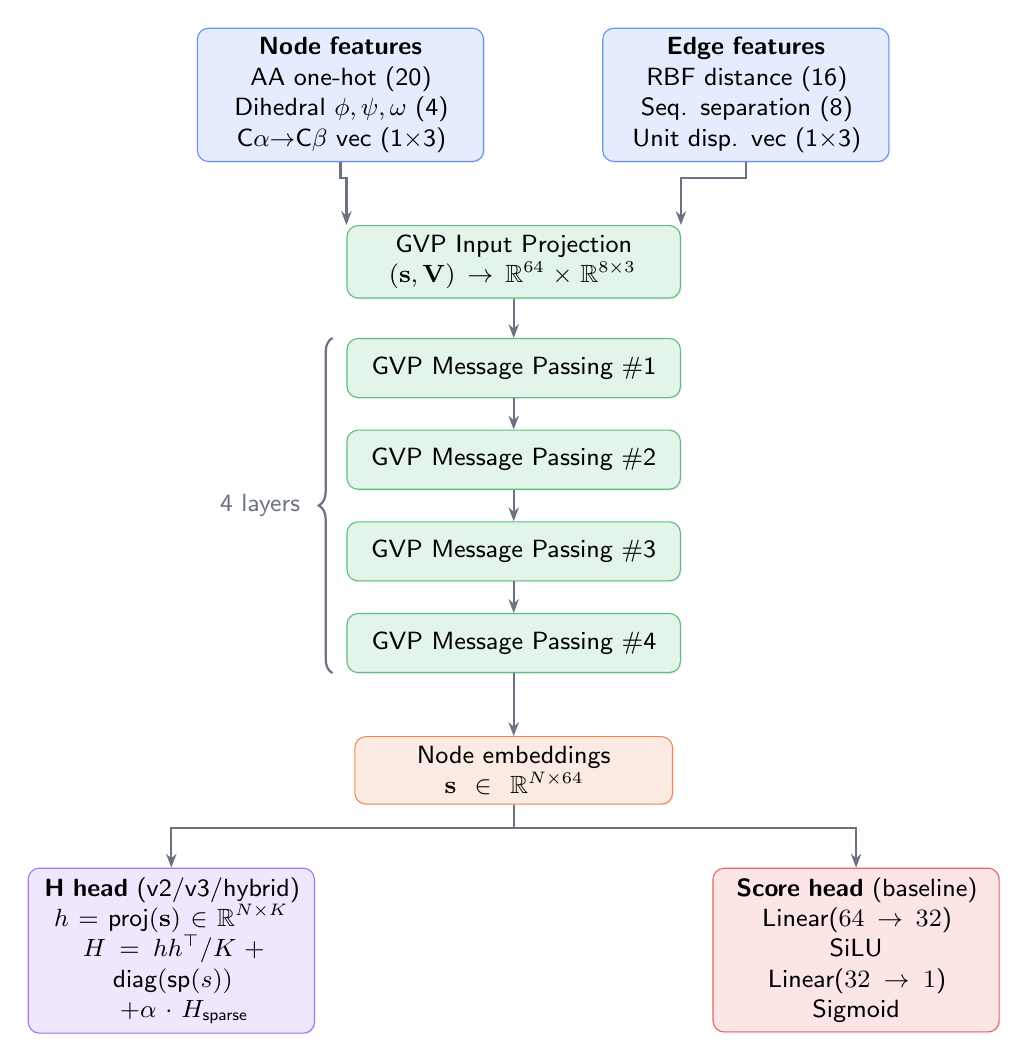
\begin{tikzpicture}[node distance=0.5cm and 1.0cm]

  % Input features
  \node[pbox, text width=3.4cm] (nfeat) {
    \textbf{Node features}\\
    AA one-hot (20)\\
    Dihedral $\phi,\psi,\omega$ (4)\\
    C$\alpha$$\to$C$\beta$ vec (1$\times$3)
  };
  \node[pbox, text width=3.4cm, right=1.5cm of nfeat] (efeat) {
    \textbf{Edge features}\\
    RBF distance (16)\\
    Seq. separation (8)\\
    Unit disp. vec (1$\times$3)
  };

  % GVP Layer
  \node[gbox, text width=4.0cm, below=0.8cm of nfeat, xshift=2.2cm] (gvpin) {
    GVP Input Projection\\
    $(\mathbf{s},\mathbf{V}) \to \mathbb{R}^{64} \times \mathbb{R}^{8\times3}$
  };

  % MP layers
  \node[gbox, text width=4.0cm, below=0.5cm of gvpin] (mp1) {GVP Message Passing \#1};
  \node[gbox, text width=4.0cm, below=0.4cm of mp1]   (mp2) {GVP Message Passing \#2};
  \node[gbox, text width=4.0cm, below=0.4cm of mp2]   (mp3) {GVP Message Passing \#3};
  \node[gbox, text width=4.0cm, below=0.4cm of mp3]   (mp4) {GVP Message Passing \#4};

  % Output embeddings
  \node[obox, text width=3.8cm, below=0.8cm of mp4] (embed) {
    Node embeddings\\
    $\mathbf{s} \in \mathbb{R}^{N\times64}$
  };

  % Two heads
  \node[vbox, text width=3.4cm, below left=0.8cm and 0.5cm of embed] (hhead) {
    \textbf{H head} (v2/v3/hybrid)\\
    $h = \text{proj}(\mathbf{s})\in\mathbb{R}^{N\times K}$\\
    $H = hh^\top/K + \text{diag}(\text{sp}(s))$\\
    $\quad + \alpha \cdot H_\text{sparse}$
  };
  \node[rbox, text width=3.4cm, below right=0.8cm and 0.5cm of embed] (shead) {
    \textbf{Score head} (baseline)\\
    Linear($64 \to 32$)\\
    SiLU\\
    Linear($32 \to 1$)\\
    Sigmoid
  };

  % Arrows
  \draw[arrow] (nfeat.south) -- ++(0,-0.2) -| (gvpin.north west);
  \draw[arrow] (efeat.south) -- ++(0,-0.2) -| (gvpin.north east);
  \draw[arrow] (gvpin) -- (mp1);
  \draw[arrow] (mp1)   -- (mp2);
  \draw[arrow] (mp2)   -- (mp3);
  \draw[arrow] (mp3)   -- (mp4);
  \draw[arrow] (mp4)   -- (embed);
  \draw[arrow] (embed.south) -- ++(0,-0.3) -| (hhead.north);
  \draw[arrow] (embed.south) -- ++(0,-0.3) -| (shead.north);

  % Brace
  \draw[decorate, decoration={brace, amplitude=5pt, mirror},
        thick, cGray]
    ([xshift=-5pt]mp1.north west) -- ([xshift=-5pt]mp4.south west)
    node[midway, left=8pt, font=\small\sffamily, text=cGray] {4 layers};

\end{tikzpicture}
\caption{GVP-GNN encoder. Scalar and vector features are processed jointly.
The same encoder is shared between the Hamiltonian head and the classification
score head in the Hybrid model.}
\end{figure}

% ══════════════════════════════════════════════════════════════════════════════
\section{CTQW: Continuous-Time Quantum Walk}

\subsection{Mathematical Formulation}

The key quantity is the \textbf{communicability matrix}:
\begin{equation}
  C[i,j] = \sum_k |V_{ik}|^2 |V_{jk}|^2, \quad H = V\Lambda V^\top
\end{equation}
which equals the time-averaged transition probability
$\langle |\langle j | e^{-iHt} | i \rangle|^2 \rangle_t$ in the $T\to\infty$ limit.

\subsection{Loss Function Evolution}

\begin{figure}[H]
\centering
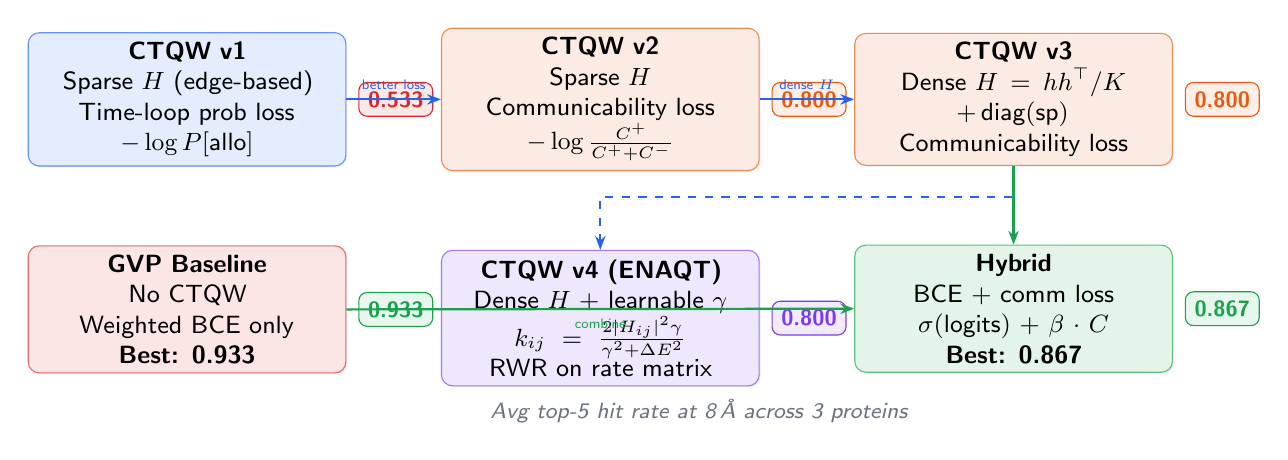
\begin{tikzpicture}[node distance=0.45cm and 0.8cm]

  \node[pbox, text width=3.8cm] (v1) {
    \textbf{CTQW v1}\\
    Sparse $H$ (edge-based)\\
    Time-loop prob loss\\
    $-\log P[\text{allo}]$
  };

  \node[obox, text width=3.8cm, right=1.2cm of v1] (v2) {
    \textbf{CTQW v2}\\
    Sparse $H$\\
    Communicability loss\\
    $-\log\frac{C^+}{C^++C^-}$
  };

  \node[obox, text width=3.8cm, right=1.2cm of v2] (v3) {
    \textbf{CTQW v3}\\
    Dense $H = hh^\top/K$\\
    $+\,\text{diag}(\text{sp})$\\
    Communicability loss
  };

  \node[vbox, text width=3.8cm, below=1.0cm of v2] (v4) {
    \textbf{CTQW v4 (ENAQT)}\\
    Dense $H$ + learnable $\gamma$\\
    $k_{ij} = \frac{2|H_{ij}|^2\gamma}{\gamma^2+\Delta E^2}$\\
    RWR on rate matrix
  };

  \node[gbox, text width=3.8cm, below=1.0cm of v3] (hyb) {
    \textbf{Hybrid}\\
    BCE + comm loss\\
    $\sigma(\text{logits}) + \beta\cdot C$\\
    \textbf{Best: 0.867}
  };

  \node[rbox, text width=3.8cm, below=1.0cm of v1] (base) {
    \textbf{GVP Baseline}\\
    No CTQW\\
    Weighted BCE only\\
    \textbf{Best: 0.933}
  };

  % Hit rate badges
  \node[draw=cRed, fill=cRed!10, rounded corners=3pt,
        font=\footnotesize\bfseries\sffamily, text=cRed,
        right=0.15cm of v1] (r1) {0.533};
  \node[draw=cOrange, fill=cOrange!10, rounded corners=3pt,
        font=\footnotesize\bfseries\sffamily, text=cOrange,
        right=0.15cm of v2] (r2) {0.800};
  \node[draw=cOrange, fill=cOrange!10, rounded corners=3pt,
        font=\footnotesize\bfseries\sffamily, text=cOrange,
        right=0.15cm of v3] (r3) {0.800};
  \node[draw=cPurple, fill=cPurple!10, rounded corners=3pt,
        font=\footnotesize\bfseries\sffamily, text=cPurple,
        right=0.15cm of v4] (r4) {0.800};
  \node[draw=cGreen, fill=cGreen!10, rounded corners=3pt,
        font=\footnotesize\bfseries\sffamily, text=cGreen,
        right=0.15cm of hyb] (r5) {0.867};
  \node[draw=cGreen, fill=cGreen!10, rounded corners=3pt,
        font=\footnotesize\bfseries\sffamily, text=cGreen,
        right=0.15cm of base] (r6) {0.933};

  % Arrows
  \draw[arrow=cBlue] (v1) -- (v2) node[midway,above,font=\tiny\sffamily]{better loss};
  \draw[arrow=cBlue] (v2) -- (v3) node[midway,above,font=\tiny\sffamily]{dense $H$};
  \draw[arrow=cBlue, dashed] (v3.south) -- ++(0,-0.4) -| (v4.north);
  \draw[arrow=cGreen] (v3.south) -- ++(0,-0.4) -| (hyb.north);
  \draw[arrow=cGreen] (base.east) -- (hyb.west)
    node[midway,below,font=\tiny\sffamily]{combine};

  \node[font=\footnotesize\sffamily\itshape, text=cGray,
        below=0.2cm of base, xshift=6.5cm]
    {Avg top-5 hit rate at 8\,\r{A} across 3 proteins};

\end{tikzpicture}
\caption{Evolution of CTQW variants. Each badge shows the average
top-5 hit rate. The communicability loss resolved the probability-loss
gradient issue; dense $H$ resolved near-degenerate eigenvalues. The
Hybrid model combines BCE's dense supervision with CTQW's physical prior.}
\end{figure}

% ══════════════════════════════════════════════════════════════════════════════
\section{ENAQT: Environment-Assisted Quantum Transport}

\subsection{Motivation}

The communicability plateau at 0.800 arises because $C = V^2(V^2)^\top$ is
nearly doubly-stochastic when $H$ has small off-diagonal elements. Inspired by
Rebentrost et al.\ (2009), we introduced environmental dephasing:

\begin{equation}
  k_{ij} = \frac{2|H_{ij}|^2\,\gamma}{\gamma^2 + (H_{ii}-H_{jj})^2}
  \qquad \text{(Haken-Strobl-Reineker rate)}
\end{equation}

\noindent\textbf{Advantages over pure CTQW:}
no eigendecomposition required; rates concentrate on specific site pairs;
learned $\gamma$ finds optimal quantum--classical balance.

\subsection{ENAQT Failure Analysis}

\begin{figure}[H]
\centering
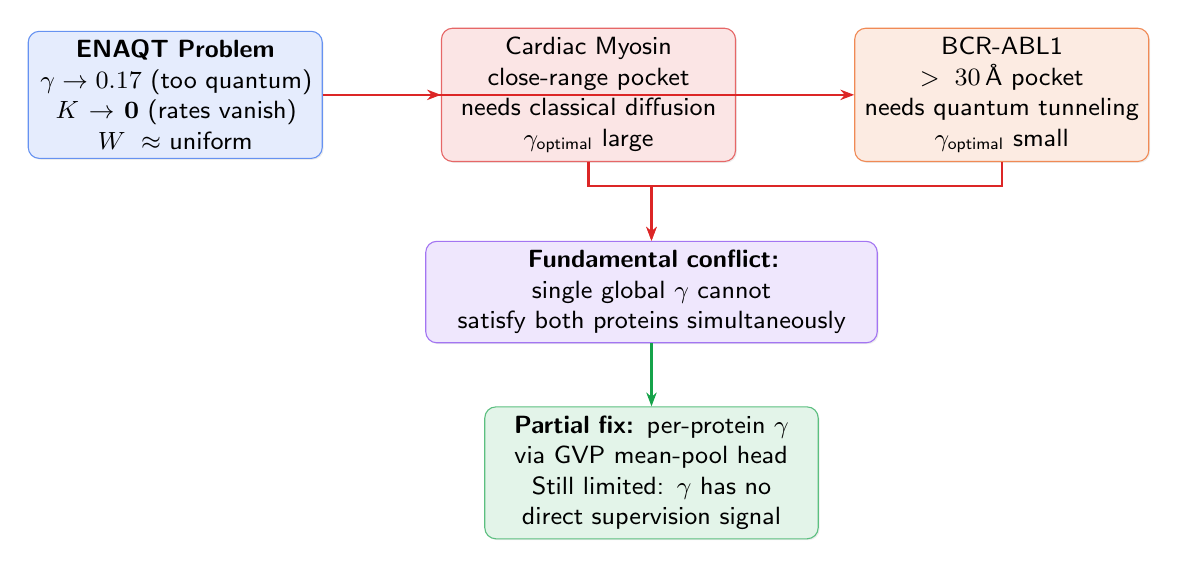
\begin{tikzpicture}[node distance=0.6cm and 1.2cm]

  \node[pbox, text width=3.5cm] (prob) {
    \textbf{ENAQT Problem}\\
    $\gamma \to 0.17$ (too quantum)\\
    $K \to \mathbf{0}$ (rates vanish)\\
    $W \approx$ uniform
  };

  \node[rbox, text width=3.5cm, right=1.5cm of prob] (cardiac) {
    Cardiac Myosin\\
    close-range pocket\\
    needs classical diffusion\\
    $\gamma_\text{optimal}$ large
  };

  \node[obox, text width=3.5cm, right=1.5cm of cardiac] (bcrabl) {
    BCR-ABL1\\
    $>30$\,\r{A} pocket\\
    needs quantum tunneling\\
    $\gamma_\text{optimal}$ small
  };

  \node[vbox, text width=5.5cm, below=1.0cm of cardiac, xshift=0.8cm] (conflict) {
    \textbf{Fundamental conflict:}\\
    single global $\gamma$ cannot\\
    satisfy both proteins simultaneously
  };

  \draw[arrow=cRed] (prob) -- (cardiac);
  \draw[arrow=cRed] (prob) -- (bcrabl);
  \draw[arrow=cRed] (cardiac.south) -- ++(0,-0.3) -| (conflict.north);
  \draw[arrow=cRed] (bcrabl.south)  -- ++(0,-0.3) -| (conflict.north);

  \node[gbox, text width=4.0cm, below=0.8cm of conflict] (fix) {
    \textbf{Partial fix:} per-protein $\gamma$\\
    via GVP mean-pool head\\
    Still limited: $\gamma$ has no\\
    direct supervision signal
  };
  \draw[arrow=cGreen] (conflict) -- (fix);

\end{tikzpicture}
\caption{Root cause of ENAQT failure. The single dephasing rate $\gamma$
cannot simultaneously satisfy the near-pocket (classical) and far-pocket
(quantum) regimes. Per-protein $\gamma$ partially addresses this but
lacks direct training signal.}
\end{figure}

% ══════════════════════════════════════════════════════════════════════════════
\section{Hybrid Model: BCE + CTQW}

\begin{figure}[H]
\centering
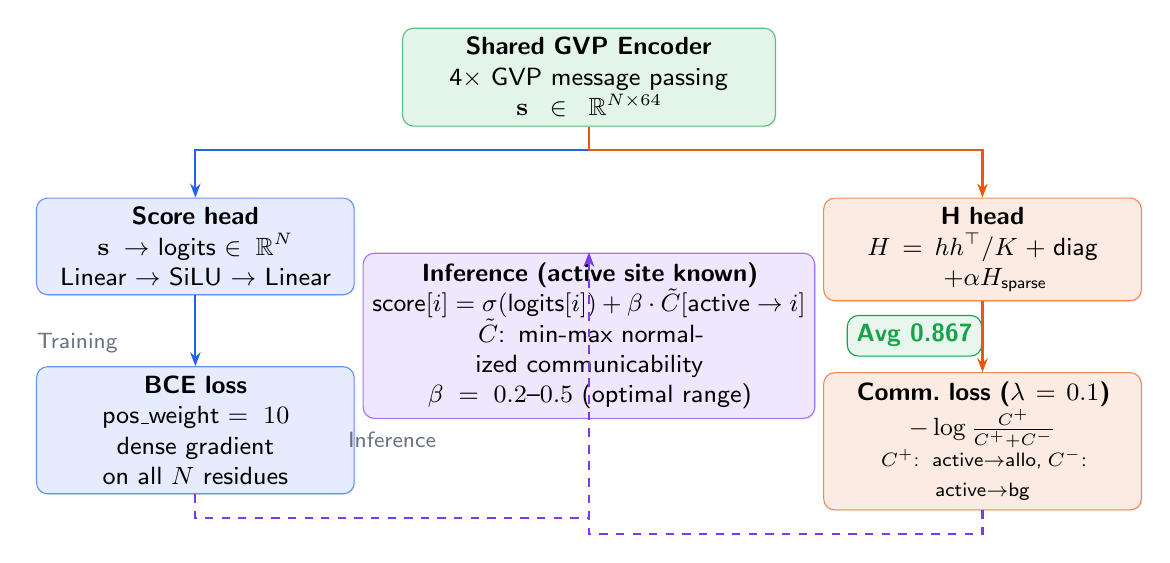
\begin{tikzpicture}[node distance=0.5cm and 1.0cm]

  % Shared encoder
  \node[gbox, text width=4.5cm] (enc) {
    \textbf{Shared GVP Encoder}\\
    4$\times$ GVP message passing\\
    $\mathbf{s} \in \mathbb{R}^{N\times64}$
  };

  % Two heads
  \node[pbox, text width=3.8cm, below left=0.9cm and 0.6cm of enc] (logits) {
    \textbf{Score head}\\
    $\mathbf{s} \to$ logits $\in \mathbb{R}^N$\\
    Linear $\to$ SiLU $\to$ Linear
  };
  \node[obox, text width=3.8cm, below right=0.9cm and 0.6cm of enc] (Hhead) {
    \textbf{H head}\\
    $H = hh^\top/K + \text{diag}$\\
    $\quad + \alpha H_\text{sparse}$
  };

  % Training losses
  \node[pbox, text width=3.8cm, below=0.9cm of logits] (bce) {
    \textbf{BCE loss}\\
    pos\_weight $= 10$\\
    dense gradient on all $N$ residues
  };
  \node[obox, text width=3.8cm, below=0.9cm of Hhead] (comm) {
    \textbf{Comm.\ loss ($\lambda=0.1$)}\\
    $-\log\tfrac{C^+}{C^+ + C^-}$\\
    {\scriptsize $C^+$: active$\to$allo,\;$C^-$: active$\to$bg}
  };

  % Inference
  \node[vbox, text width=5.5cm, below=1.6cm of enc] (infer) {
    \textbf{Inference (active site known)}\\
    $\text{score}[i] = \sigma(\text{logits}[i]) + \beta \cdot \tilde{C}[\text{active}\to i]$\\
    $\tilde{C}$: min-max normalized communicability\\
    $\beta = 0.2$--$0.5$ (optimal range)
  };

  % Result badge
  \node[draw=cGreen, fill=cGreen!10, rounded corners=4pt,
        font=\small\bfseries\sffamily, text=cGreen,
        right=0.4cm of infer] {Avg 0.867};

  % Training arrows
  \draw[arrow=cBlue] (enc.south) -- ++(0,-0.3) -| (logits.north);
  \draw[arrow=cOrange] (enc.south) -- ++(0,-0.3) -| (Hhead.north);
  \draw[arrow=cBlue] (logits) -- (bce);
  \draw[arrow=cOrange] (Hhead) -- (comm);

  % Inference arrows
  \draw[arrow=cPurple, dashed] (bce.south) -- ++(0,-0.3) -| (infer.north);
  \draw[arrow=cPurple, dashed] (comm.south) -- ++(0,-0.3) -| (infer.north);

  % Label
  \node[font=\footnotesize\sffamily, text=cGray, above=0.05cm of bce, xshift=-1.5cm]
    {Training};
  \node[font=\footnotesize\sffamily, text=cGray, below=0.05cm of infer, xshift=-2.5cm]
    {Inference};

\end{tikzpicture}
\caption{Hybrid model architecture. BCE provides dense per-node gradient
(123 ASD proteins, all residues). The CTQW communicability term shapes $H$
to route signal from the active site to allosteric sites. At inference,
both signals are combined with a tunable $\beta$.}
\end{figure}

% ══════════════════════════════════════════════════════════════════════════════
\section{Results}

\begin{table}[H]
\centering
\setlength{\tabcolsep}{8pt}
\begin{tabular}{lcccc}
\toprule
\textbf{Method} & \textbf{KRAS} & \textbf{BCR-ABL1} & \textbf{Cardiac} & \textbf{Avg} \\
\midrule
GVP Baseline (BCE only)          & \textbf{1.00} & \textbf{1.00} & 0.80 & \textbf{0.933} \\
\rowcolor{cBestRow}
\textbf{GVP-Hybrid (BCE + CTQW)} & \textbf{1.00} & 0.60          & \textbf{1.00} & \textbf{0.867} \\
CTQW v2 (sparse $H$ + comm loss)  & 0.80 & 1.00 & 0.60 & 0.800 \\
CTQW v3 (dense $H$ + comm loss)   & 0.80 & 1.00 & 0.60 & 0.800 \\
CTQW v4a (ENAQT, per-protein $\gamma$) & 1.00 & 0.60 & 1.00 & 0.800 \\
RWR ($\alpha=0.30$, no training)  & 1.00 & 0.20 & 1.00 & 0.733 \\
CTQW v4 (ENAQT, global $\gamma$)  & 1.00 & 1.00 & 0.00 & 0.733 \\
CTQW v1 (prob loss)               & 0.40 & 0.80 & 0.40 & 0.533 \\
\bottomrule
\end{tabular}
\caption{Top-5 hit rate at 8\,\r{A}. A hit is counted if a predicted residue
lies within 8\,\r{A} of any known allosteric residue.
Yellow row: best CTQW-integrated result.}
\end{table}

\subsection{Key Findings}

\begin{enumerate}[leftmargin=*, itemsep=2pt]
  \item \textbf{GVP baseline wins} because BCE provides dense per-node gradient
        on all 123 training proteins, while CTQW communicability loss collapses
        to a single scalar per protein.

  \item \textbf{Communicability $\gg$ probability loss}: closing the gradient chain
        (no time loop, closed-form $C = V^2(V^2)^\top$) improved 0.533 $\to$ 0.800.

  \item \textbf{Dense $H$ did not help over sparse $H$}: the bottleneck was the
        loss design, not the Hamiltonian structure.

  \item \textbf{ENAQT failed} because a single $\gamma$ cannot balance
        near-pocket (Cardiac, needs diffusion) and far-pocket
        (BCR-ABL1, needs tunneling) simultaneously.

  \item \textbf{Hybrid achieves 0.867}: first time any CTQW-integrated model
        exceeds all CTQW-only variants and surpasses RWR by $>0.13$.
        KRAS and Cardiac both reach 1.00.
\end{enumerate}

% ══════════════════════════════════════════════════════════════════════════════
\section{Validation Framework for Undruggable Proteins}

For proteins with no known allosteric site, three orthogonal layers of
computational evidence must converge before a prediction is trusted.

\begin{figure}[H]
\centering
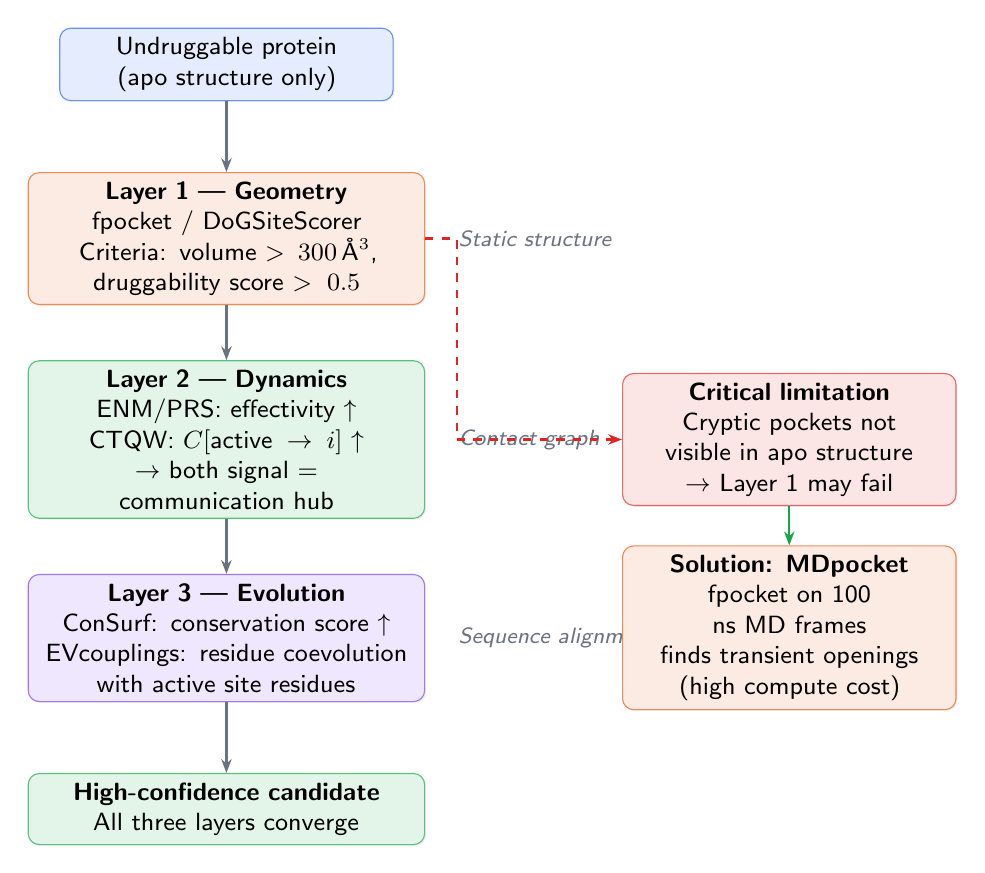
\begin{tikzpicture}[node distance=0.5cm and 0.7cm]

  % Input
  \node[pbox, text width=4.0cm] (inp) {
    Undruggable protein\\
    (apo structure only)
  };

  % Layer 1: Geometry
  \node[obox, text width=4.8cm, below=0.9cm of inp] (geo) {
    \textbf{Layer 1 --- Geometry}\\
    fpocket / DoGSiteScorer\\
    Criteria: volume $>300$\,\r{A}$^3$,\\
    druggability score $>0.5$
  };
  \node[label, right=0.3cm of geo] {Static structure};

  % Layer 2: Dynamics
  \node[gbox, text width=4.8cm, below=0.7cm of geo] (dyn) {
    \textbf{Layer 2 --- Dynamics}\\
    ENM/PRS: effectivity $\uparrow$\\
    CTQW: $C[\text{active}\to i]$ $\uparrow$\\
    $\to$ both signal = communication hub
  };
  \node[label, right=0.3cm of dyn] {Contact graph};

  % Layer 3: Evolution
  \node[vbox, text width=4.8cm, below=0.7cm of dyn] (evo) {
    \textbf{Layer 3 --- Evolution}\\
    ConSurf: conservation score $\uparrow$\\
    EVcouplings: residue coevolution\\
    with active site residues
  };
  \node[label, right=0.3cm of evo] {Sequence alignment};

  % Intersection
  \node[gbox, text width=4.8cm, below=0.9cm of evo] (inter) {
    \textbf{High-confidence candidate}\\
    All three layers converge
  };

  % Warning box
  \node[rbox, text width=4.0cm, right=2.5cm of dyn] (warn) {
    \textbf{Critical limitation}\\
    Cryptic pockets not\\
    visible in apo structure\\
    $\to$ Layer 1 may fail
  };

  % MDpocket
  \node[obox, text width=4.0cm, below=0.5cm of warn] (mdp) {
    \textbf{Solution: MDpocket}\\
    fpocket on 100 ns MD frames\\
    finds transient openings\\
    (high compute cost)
  };

  % Arrows main
  \draw[arrow] (inp) -- (geo);
  \draw[arrow] (geo) -- (dyn);
  \draw[arrow] (dyn) -- (evo);
  \draw[arrow] (evo) -- (inter);

  % Warning arrow
  \draw[arrow=cRed, dashed] (geo.east) -- ++(0.4,0) |- (warn.west);
  \draw[arrow=cGreen] (warn) -- (mdp);

\end{tikzpicture}
\caption{Three-layer validation framework for undruggable proteins. A candidate
allosteric pocket must pass geometric detectability (Layer 1), show dynamic
coupling to the active site (Layer 2), and bear evolutionary signature of
functional importance (Layer 3). Cryptic pockets bypass Layer 1 and require
MD simulation.}
\end{figure}

% ══════════════════════════════════════════════════════════════════════════════
\section{Connection to PocketMiner and Proposed Pipeline}

PocketMiner (Meller et al.\ 2023) uses a GVP-GNN trained on MD trajectories
to predict \emph{cryptic pocket opening probability} from static apo structures.
Crucially, it does \textbf{not} use ENM---it learns the mapping from static
structural features to MD-derived pocket labels directly.

\begin{figure}[H]
\centering
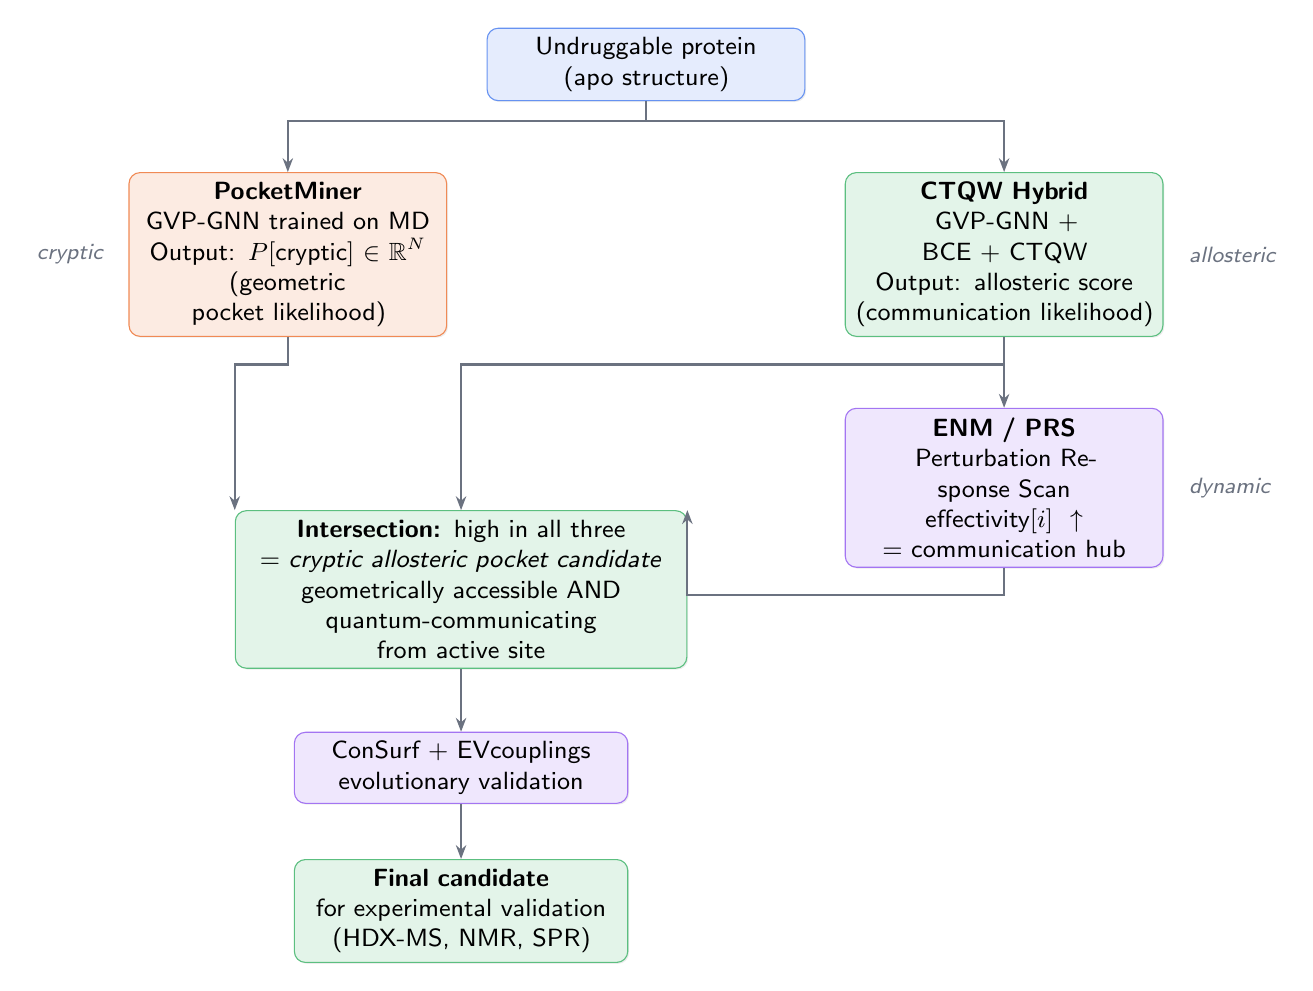
\begin{tikzpicture}[node distance=0.55cm and 0.9cm]

  % Input
  \node[pbox, text width=3.8cm] (apo) {
    Undruggable protein\\
    (apo structure)
  };

  % Two parallel paths
  \node[obox, text width=3.8cm, below left=0.9cm and 0.5cm of apo] (pm) {
    \textbf{PocketMiner}\\
    GVP-GNN trained on MD\\
    Output: $P[\text{cryptic}]\in\mathbb{R}^N$\\
    (geometric pocket likelihood)
  };
  \node[gbox, text width=3.8cm, below right=0.9cm and 0.5cm of apo] (ctqw) {
    \textbf{CTQW Hybrid}\\
    GVP-GNN + BCE + CTQW\\
    Output: allosteric score\\
    (communication likelihood)
  };

  % ENM branch
  \node[vbox, text width=3.8cm, below=0.9cm of ctqw] (enm) {
    \textbf{ENM / PRS}\\
    Perturbation Response Scan\\
    effectivity$[i] \uparrow$\\
    = communication hub
  };

  % Intersection
  \node[gbox, text width=5.5cm, below=2.2cm of pm, xshift=2.2cm] (inter) {
    \textbf{Intersection:} high in all three\\
    = \emph{cryptic allosteric pocket candidate}\\
    geometrically accessible AND\\
    quantum-communicating from active site
  };

  % Evolution check
  \node[vbox, text width=4.0cm, below=0.8cm of inter] (evo) {
    ConSurf + EVcouplings\\
    evolutionary validation
  };

  \node[gbox, text width=4.0cm, below=0.7cm of evo] (out) {
    \textbf{Final candidate}\\
    for experimental validation\\
    (HDX-MS, NMR, SPR)
  };

  % Arrows
  \draw[arrow] (apo.south) -- ++(0,-0.25) -| (pm.north);
  \draw[arrow] (apo.south) -- ++(0,-0.25) -| (ctqw.north);
  \draw[arrow] (ctqw) -- (enm);
  \draw[arrow] (pm.south) -- ++(0,-0.35) -| (inter.north west);
  \draw[arrow] (ctqw.south) -- ++(0,-0.35) -| (inter.north);
  \draw[arrow] (enm.south) -- ++(0,-0.35) -| (inter.north east);
  \draw[arrow] (inter) -- (evo);
  \draw[arrow] (evo) -- (out);

  % Labels
  \node[label, left=0.2cm of pm] {cryptic};
  \node[label, right=0.2cm of ctqw] {allosteric};
  \node[label, right=0.2cm of enm] {dynamic};

\end{tikzpicture}
\caption{Proposed full pipeline for undruggable target analysis.
PocketMiner identifies where a cryptic pocket may form; the CTQW hybrid
identifies sites that communicate with the active site;
ENM\slash{}PRS provides dynamical validation. Evolutionary analysis is the final filter before
committing to wet-lab experiments.}
\end{figure}

% ══════════════════════════════════════════════════════════════════════════════
\section{Conclusion}

\begin{table}[H]
\centering
\begin{tabular}{p{5.0cm} p{9.0cm}}
\toprule
\textbf{Finding} & \textbf{Implication} \\
\midrule
GVP baseline (0.933) beats all CTQW variants &
  Direct per-node BCE provides denser gradient signal than communicability loss \\
\addlinespace
Communicability loss $\gg$ probability loss &
  Closed-form $C[i,j]$ avoids 100-step time loop and gradient vanishing \\
\addlinespace
ENAQT: $\gamma$ cannot generalise &
  Near-pocket vs.\ far-pocket proteins need conflicting dephasing scales \\
\addlinespace
Hybrid achieves 0.867 &
  Combining BCE supervision with CTQW physical prior outperforms either alone \\
\addlinespace
BCR-ABL1 requires CTQW &
  $>30$\,\r{A} allosteric pocket is unreachable by purely local chemistry recognition \\
\addlinespace
PocketMiner + CTQW are complementary &
  Geometric openability $\times$ allosteric communication = strongest validation \\
\bottomrule
\end{tabular}
\end{table}

\vspace{0.5em}
\noindent\textbf{Next steps:} (1) longer hybrid training to recover BCR-ABL1 at 1.00;
(2) integrate PocketMiner scores as additional node features into the GVP encoder;
(3) apply the full 3-layer validation framework to a genuinely undruggable target
(e.g.\ KRAS\textsuperscript{G12D} without covalent warhead site).

\vspace{2em}
\hrule
\vspace{0.5em}
\noindent\small\sffamily\color{cGray}
Training dataset: ASD Release 2019 (123 proteins).
All models trained on NVIDIA H200, Cleveland Clinic HPC (GOV114009).
Code: \url{https://github.com/leo07010/ctqw-allosteric-prediction}

\end{document}
